\section{Introduction}

In traditional classification problems, an instance $\mathbf{x}_i \in X$ can be classified in only one class $c_j \in C$. Nonetheless, there are more complex classification tasks, where an instance can be simultaneously classified into a set of classes $C_j \in C$. One of this tasks is called Hierarchical Multi-Label Classification (HMC), in which an instance can be classified into a set of classes that are previously organized as a hierarchy, with subclasses and superclasses. In this hierarchy, superclass relationships are represented by a partial order $\prec_h$, \emph{i.e.}, for all $c_1, c_2 \in C, c_1 \prec_h c_2$ if and only if $c_1$ is a superclass of $c_2$.

Protein Function Prediction (PFP) is one of the most important applications related to HMC, because proteins perform many important functions within an organism. Proteins are related to biochemical reactions, cell signaling, structural, and mechanical functions~\cite{Costa2008}, to name a few. Given that protein functions are hierarchically related, PFP can be considered a typical HMC problem.

In this work, we make use of the Gene Ontology (GO) hierarchy to investigate the PFP problem. In the GO, classes are organized as a Directed Acyclic Graph (DAG) hierarchy of terms, in which each term corresponds to a protein function. The hierarchy comprises three ontologies covering different domains, each one with thousands of classes: {\it cellular components}, {\it biological processes}, and {\it molecular functions}~\cite{Ashburner2000}. Figure~\ref{fig:GO} illustrates a small part of the GO taxonomy.

\begin{figure*}[ht]
    \centering
    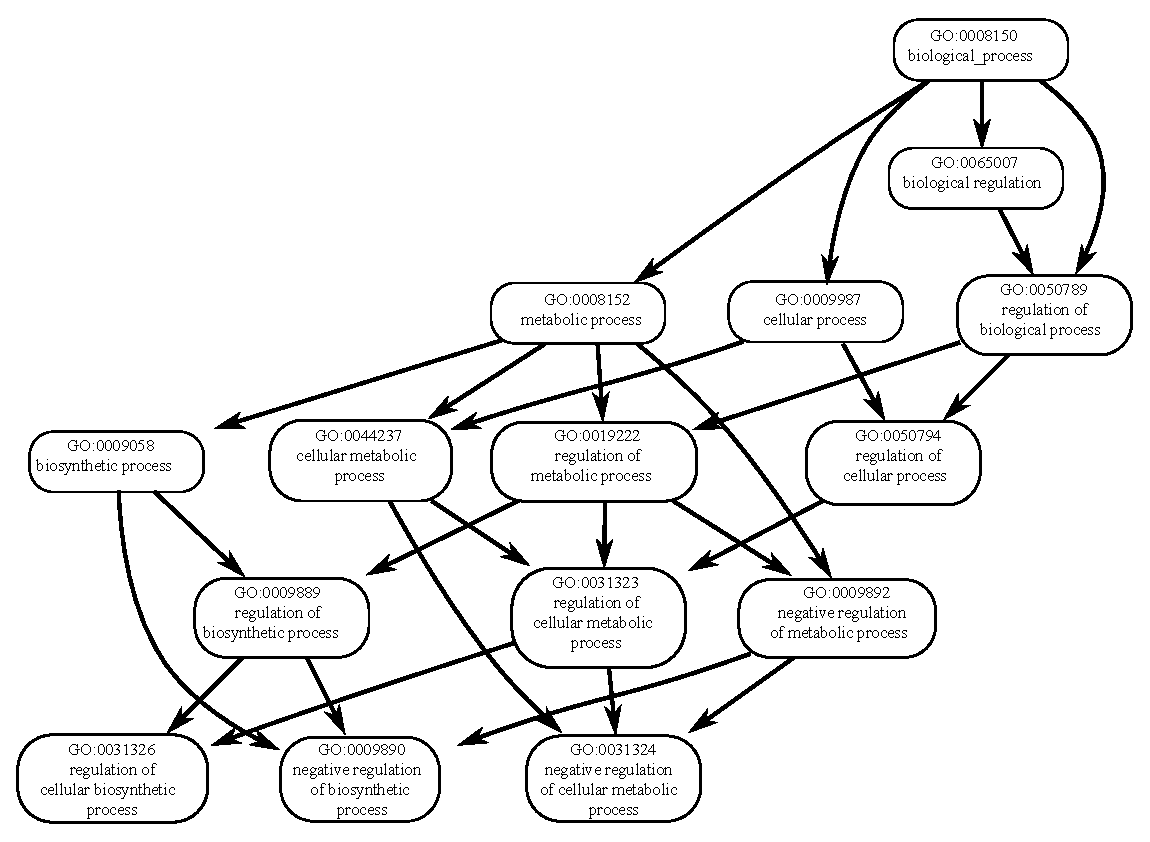
\includegraphics[scale=0.7]{GO-Taxonomy}
    \caption{Part of the Gene Ontology Hierarchical Taxonomy. (Adapted from Ashburner et. al. \cite{Ashburner2000})}
    \label{fig:GO}
\end{figure*}

The PFP task using the GO taxonomy is a very challenging problem. As we traverse the hierarchy down to the leaves, making accurate predictions becomes more difficult since terms have fewer and fewer positive instances. In addition, instances can be classified simultaneously into two or more paths of the hierarchy, and a term can have more than one parent node. We work with the ``is-a'' relation, which forms the basic structure of the GO. Thus, A is a B means that term A is a subtype of term B. Also, classifying an instance into class $c_j$ means that we are classifying it into all superclasses of class $c_j$. This is the multiple inheritance interpretation, which is the correct interpretation when working with the GO~\cite{Ashburner2000}.

%Two approaches have been used to solve HMC problems: local and global. In the local approach, conventional classification algorithms, such as decision tree induction algorithms or support vector machines, are trained to produce a hierarchy of classifiers. A classification for a new instance is then obtained combining the predictions provided by the individual classifiers~\cite{Costa2007}. In this approach, local information about the class hierarchy is used during the induction of each base classifier. According to \cite{Silla2010}, this local information can be used in different ways, depending on how the local classifiers are induced. The three main strategies for using local information are: one Local Classifier per Node (LCN), one Local Classifier per Parent Node (LCPN), and one Local Classifier per Level (LCL). The LCN strategy trains one binary classifier for each class of the hierarchy \cite{Valentini2009}. The LCPN strategy  trains, for each internal class, a multi-class classifier to distinguish between its subclasses \cite{Svetlana2004}, and the LCL strategy trains one multi-class classifier for each hierarchical level, where each classifier is responsible for the prediction in its associated level~\cite{Cerri2013}.

%Different from the local approach, the global approach induces a single classifier using all classes of the hierarchy at once. After the training process, the classification of a new instance by the induced classifier occurs in just one step \cite{Vens2008}. As global methods induce a single classifier to consider the specificities of the classification problem, they usually do not make use of conventional classification algorithms, unless these are adapted to consider the hierarchy of classes~\cite{Otero2010}.

The novel contributions of this paper are as follows. First, we propose a method called {\bf H}ierarchical {\bf M}ulti-Label {\bf C}lassification with {\bf L}ocal {\bf M}ulti-{\bf L}ayer {\bf P}erceptron (HMC-LMLP), which associates an MLP to each level of the hierarchy, in which each MLP is responsible for the predictions in its associated level. A very preliminary version of HMC-LMLP has been reported in \cite{Cerri2013}. Differently from the version in \cite{Cerri2013}, we employ the labels of the training instances as part of the input to train each MLP. Therefore, when training an MLP for level $l$, the feature vector of an instance is augmented with its classes for the level $l-1$. With this modification, we try to enforce the label dependencies between classes to be taken into account. We also propose a second version which ignores the labels associated with the classes to augment the feature vectors of the instances. This can be considered as a baseline version that allows us to examine whether the use of the labels to augment the feature vectors results in performance improvement.

Second, we employ the Local Classifier per Level (LCL)~\cite{Silla2010} strategy to make use of local information within each level of the hierarchy. By using one classifier per level we do not decompose the classification problem into a large number of sub-problems. The use of many classifiers per level may result in the application of over-specific local information, loss of important information, and loss of label dependency during training~\cite{Silla2010}. Finally, we present an analysis of the application of the LCL strategy to DAG-structured class hierarchies, adapting the DAG structure datasets in order to use them in the experiments. %Verifying the performance of the LCL strategy in very deep hierarchies with thousands of classes and class relationships is of great interest to researchers working with HMC problems.

%by using the LCL strategy, we intend to avoid deficiencies of both local and global methods. Unlike the global approach, HMC-LMLP is able to use local information which can be very useful to explore different data patterns in distinct hierarchical levels. Also, differently from the LCN and LCPN strategies, HMC-LMLP does not decompose the classification problem into a large number of sub-problems. The use of many classifiers per level may result in the application of over-specific local information, loss of important information, and loss of label dependency during training~\cite{Silla2010}. 

The remainder of this paper is organized as follows. Section~\ref{sec:relatedWork} presents related work regarding HMC for PFP. The proposed HMC-LMLP method is detailed in Section~\ref{sec:HMC-LMLP}, whereas a thorough empirical analysis is carried out in Section~\ref{sec:experiments}. A deeper discussion on the results is performed in Section~\ref{sec:discussion}, and the final considerations and future research directions are presented in Section~\ref{sec:conclusion}.

